\documentclass[oneside]{book}
\usepackage[utf8]{inputenc}
\usepackage{graphicx}
\usepackage{geometry}
\usepackage{float}
\usepackage{textcomp}
\usepackage{gensymb}
\usepackage{amsmath}
\usepackage{listings}
\geometry{portrait, margin=1. in}
\usepackage[colorlinks = true,
            linkcolor = blue,
            urlcolor  = blue,
            citecolor = blue,
            anchorcolor = blue]{hyperref}
            
\usepackage{times}
\usepackage{textcomp}


\newcommand{\DVEP}{DV$\pi$P }
\newcommand{\QS}{Q$^2$}
\newcommand{\DST}{\href{https://clasweb.jlab.org/wiki/index.php/CLAS12_DSTs}{CLAS12 DST Documentation }}
\newcommand{\XB}{x$_B$}
\newcommand{\phit}{$\phi$}
\newcommand{\rexn}{$e + p \rightarrow e' + p' + \pi^0$ }
\newcommand{\vpp}{$\Gamma$(\QS , \XB)}


\newcommand{\comtilde}{\~}
%\usepackage{textcomp}
%\newcommand{\textapprox}{\raisebox{0.5ex}{\texttildelow}}
\lstset{language=Python}
\lstset{frame=lines}
%\lstset{caption={Insert code directly in your document}}
%\lstset{label={lst:code_direct}}
\lstset{basicstyle=\footnotesize}

\title{CLAS12 \DVEP Analysis Note}
\author{R. Johnston}
\date{\today}



\begin{document}
\maketitle
Note: This document is available online \href{https://latexonline.cc/compile?git=https\%3A\%2F\%2Fgithub.com\%2Frobertej19\%2FClas12AnaNote&target=main.tex&command=pdflatex\&trackId=1593973491329}{here}. It is a work in progress, and as of July 2020 is in its very early stages. It is continuously synchronized with its source overleaf document. For access to the source overleaf page, contact robertej@mit.edu. Code for this project can be found at \href{https://github.com/robertej19/analysis_code/projects/1
}{my repository}.


\iffalse
\chapter{Personal To Do}


\section{Introduction}
Need to make plan!
Make tentative outline of how it will go to get a cross section
Define issues, etc
Push forward
It’s a question of the uncertainties 
What do we need to get cross sections by the end of the year using some subset of the data and some subset of the cross sections

Is it possible to show the same type graphs, but as a function of the t variable. Also, even more interesting would be, a two dimensional graphs  showing the distributions of events vs Q2 and t  for a given W, e.g. 3 GeV, for both the forward and central detectors.\\

Run through the 174 inbending runs\\

How does analysis change when using custom cuts instead of normal event builder cuts?\\


Make previous plots all broken up on fd and cd, and without using proton momentum\\

Make same plot on fd on cd \\
test across all 6 sectors\\
Show missing mass plots\\
Plot train info from pid\\

Plot based for pid says it's a proton at 5 gev, see that pod is still working there, cut shouldnt be too narrow, might have kinematic constraints\\

Compare with and without proton momentum - tag it, but dont use it to measure t and phi. Different systematics, so compare proton sytematics cd to pi systematics fd\\

\fi

\section{Particle ID}
Using Event Builder Cuts:
\section{Uncertainties}
\section{Binning}
\section{Luminosity}
\section{Simulation}



\chapter{Motivation and Background}
    \input{MotBack/MotBack}
    
\chapter{CLAS12}
    \input{CLAS12Detector/CLAS12}
    
\chapter{Data Sets}
    
\begin{lstlisting}
inbending: /cache/clas12/rg-a/production/recon/fall2018/torus-1/pass1/v0/dst/train/skim8/

outbending: /volatile/clas12/rg-a/production/recon/fall2018/torus+1/pass1/v0/dst/train/skim4/

Bobby, FX has eppi0 train data, which can significantly reduce code run time at /work/clas12/fxgirod/eppi0/

\end{lstlisting}

Outbending cooking is ongoing, so there aren’t many files yet.
    
\chapter{Particle Identification}
    \input{pid/pid}
    
\chapter{Coding}
    \section{Coding notes}
\href{https://github.com/drewkenjo/dst_monitoring/wiki/Syntactic-sugar}{Syntatic Sugar}


\section{How to Enable Multi-Threading}

    \subsection{1}
        At ifarm, check if you have ~/.groovy  directory
        Otherwise create one.

    \subsection{2}
        Download Andrey’s sugar.
        
        \begin{lstlisting}
            cd ~/.groovy
            wget https://github.com/drewkenjo/dst_monitoring/releases/download/v0/sugar.jar
        \end{lstlisting}


    \subsection{3}
        The standard way to access coatjava at ifarm is adding following commands at \comtilde/.cshrc or \comtilde/.bashrc depending on which shell you use.
        
        \begin{lstlisting}
        source /group/clas12/packages/setup.csh
        module load clas12/pro
        \end{lstlisting}
        
        However, this doesn’t allow you to edit bin files.
        Simply copy run-groovy at any directory with your permission, say \comtilde/.groovy, i.e.
        
        \begin{lstlisting}
        cp $COATJAVA/bin/run-groovy ~/.groovy/
        \end{lstlisting}
        
        edit \comtilde/.groovy/run-groovy ’s line 59 from -Xmx2048m to -Xmx4096m. This will increase memory that can be used in your ifarm.
        
    \subsection{4}
        I guess you have your own standalone analysis script that runs as a main file.
        The idea is to convert this as a class, and call from other main file.
        This is not necessary for parallel computing, but this helps to run multiple analysis at one time and to maintain scripts tidy.
        
        Actually, groovy supports usage of both class and main likewise python’s ‘ if \_\_name\_\_ == “main” '.
        You can put a closure with the same name of the class. See \href{https://stackoverflow.com/questions/52543035/check-if-groovy-script-is-being-executed-directly}{here}
        
    \subsection{5}
        I have standalone analysis script epg.groovy (, which is main itself), \href{https://github.com/Sangbaek/analysis_code/blob/analysis/sangbaek/epg.groovy}{here}
        The code’s structure is like this:\\
        line 1–17: import libraries\\
        line 18–127: defining histograms\\
        line 128–319: main loop to read files (ignore line 131–154 because nowadays Nick is placing inbending and outbending in separate directories)
        line 320–384: saving histograms\\
        
        I converted that to a class file dvcs.groovy, \href{https://github.com/Sangbaek/analysis_code/blob/analysis/sangbaek/dvcs.groovy}{here}
        Here’re how-to’s.\\
        1) Add package name at line 1\\
        2) Add  import java.util.concurrent.ConcurrentHashMap at line 19\\
        3) class name at line 22. class dvcs\{ for this case\\
        4) Change histograms to be used for ConcurrentHashMap. Please compare line 24–60 of dvcs.groovy to 18–127 of epg.groovy.\\
        5) add def processEvent(event)\{ before the loop starts (line 80). The loop contents don’t have to differ from your previous main file.
        6) Remove all histogram saving steps (e.g. line 320-384 of my epg.groovy)\\
        7) Instead, you can set up your histogram's name and directory directly when you fill the histogram,
        e.g.) hists.computeIfAbsent("/epg/elec\_polar\_sec"+ele\_sec, h\_polar\_rate).fill(Math.toDegrees(ele.theta()))
        This will save histograms at /epg/elec\_polar\_sec1–/epg/elec\_polar\_sec6
        Andrey’s sugar will deal with directory structures so that you don’t have to "out.mkdir(dir); out.cd(dir); out.addDataSet(hist)” manually.
        
        By the way, with Andrey’s sugar, you can now add or subtract LorentzVector like def VmissG = beam + target - ele - pro at line 109.\\
        
    \subsection{6}
        Now download \href{https://github.com/Sangbaek/analysis_code/blob/analysis/sangbaek/run.groovy}{this}\\
        Change line 22 of run.groovy to your own class name.\\
        To run this,\\
        
        run-groovy sangbaek/run.groovy `find /cache/clas12/rg-a/production/recon/fall2018/torus-1/pass1/v0/dst/train/skim8/ -name "*.hipo”`
        
    \subsection{7}
        
        
        
        As for 3, I forgot to tell you that line 5–7 needs to be changed as
        
        \begin{lstlisting}
        CLARA_HOME=$COATJAVA/bin/..
        CLAS12DIR=$COATJAVA/bin/..
        CLAS12DIR=$COATJAVA/bin/.. ; export CLAS12DIR
        .
        
        \end{lstlisting}
        
        
        
        To use your edited run-groovy, there are two ways that I know of.\\
        
        First way is to include following line at \comtilde/.cshrc.\\
        alias run-groovy /home/sangbaek/.groovy/run-groovy\\
        
        Second one is to include following shebang line at your groovy scripts like below.\\
   
        \begin{lstlisting}     
        #!/home/sangbaek/.groovy/run-groovy\\
        \end{lstlisting}       
        
        I find the first one easier.



\chapter{Analysis Method}
    

For each kinematic bin the differential cross section can be written as:

\begin{equation}
    \sigma = \frac{N_{meas}}{L \epsilon}\frac{1}{\delta}
\end{equation}

Where $\frac{N_{meas}}{L}$ is the number of events from experiment normalized by the integrated luminosity before acceptance and radiatvie corrections. $\epsilon$ = $\frac{N^{RAD}_{rec}}{{N^{RAD}_{gen}}}$ is the acceptance correction and $\delta$ is the radiative correction.



$\delta$ can be obtained by using the following:

\begin{equation}
    \delta = \frac{N^{RAD}_{gen}}{N^{NORAD}_{gen}}
\end{equation}

luminosity = avogadros constant times the length of the target times teh density of the target (liquid hydrogen), times the ttoal collected charge in the farday cup, divided by the electron charge. 

\begin{equation}
    L = \frac{N_A l \rho Q_{FCUP}}{e}
\end{equation}
    \section{Luminosity}

The strategy to calculate the luminosity is as follows:\\

 - For each run, retrieve a measure of how much beam passed through the target, I believe in the case of CLAS12 using the Faraday cup to measure beam charge
    - sum the beam charge over all runs being considered and include any relevant corrections factors
    - multiply this by target length, density, etc. to get the integrated luminosity
    - use this value to calculate cross sections.


Implementation:

The bank REC::Event has an ?object? beamCharge, in nanoColumbs, which is described in the \DST as "beam charge integrated from the beginning of the run to the most recent reading of the gated Faraday Cup scaler in RAW::scaler, with slope/offset conversion to charge from CCDB. Note, this value will be zero in each file until the first scaler reading in that file.". This is the (un?)gated beam charge. 


This can be accessed via:

\begin{lstlisting}
	def banknames = ['REC::Event','REC::Particle','REC::Cherenkov','REC::Calorimeter','REC::Traj','REC::Track','REC::Scintillator']

	if(banknames.every{event.hasBank(it)}) {
		def (evb,partb,cc,ec,traj,trck,scib) = banknames.collect{event.getBank(it)}
def fcupBeamCharge = evb.getFloat('beamCharge',0)
\end{lstlisting}

    According to \href{https://clas12.discourse.group/t/accessing-beam-charge-information/239}{this} we might need to use tag=1 RAW::scaler::fcupgated instead of REC::Event::beamCharge
    

The beam charge needs to be converted to integrated luminosity, which can be done as follows:



\begin{figure}
    \centering
    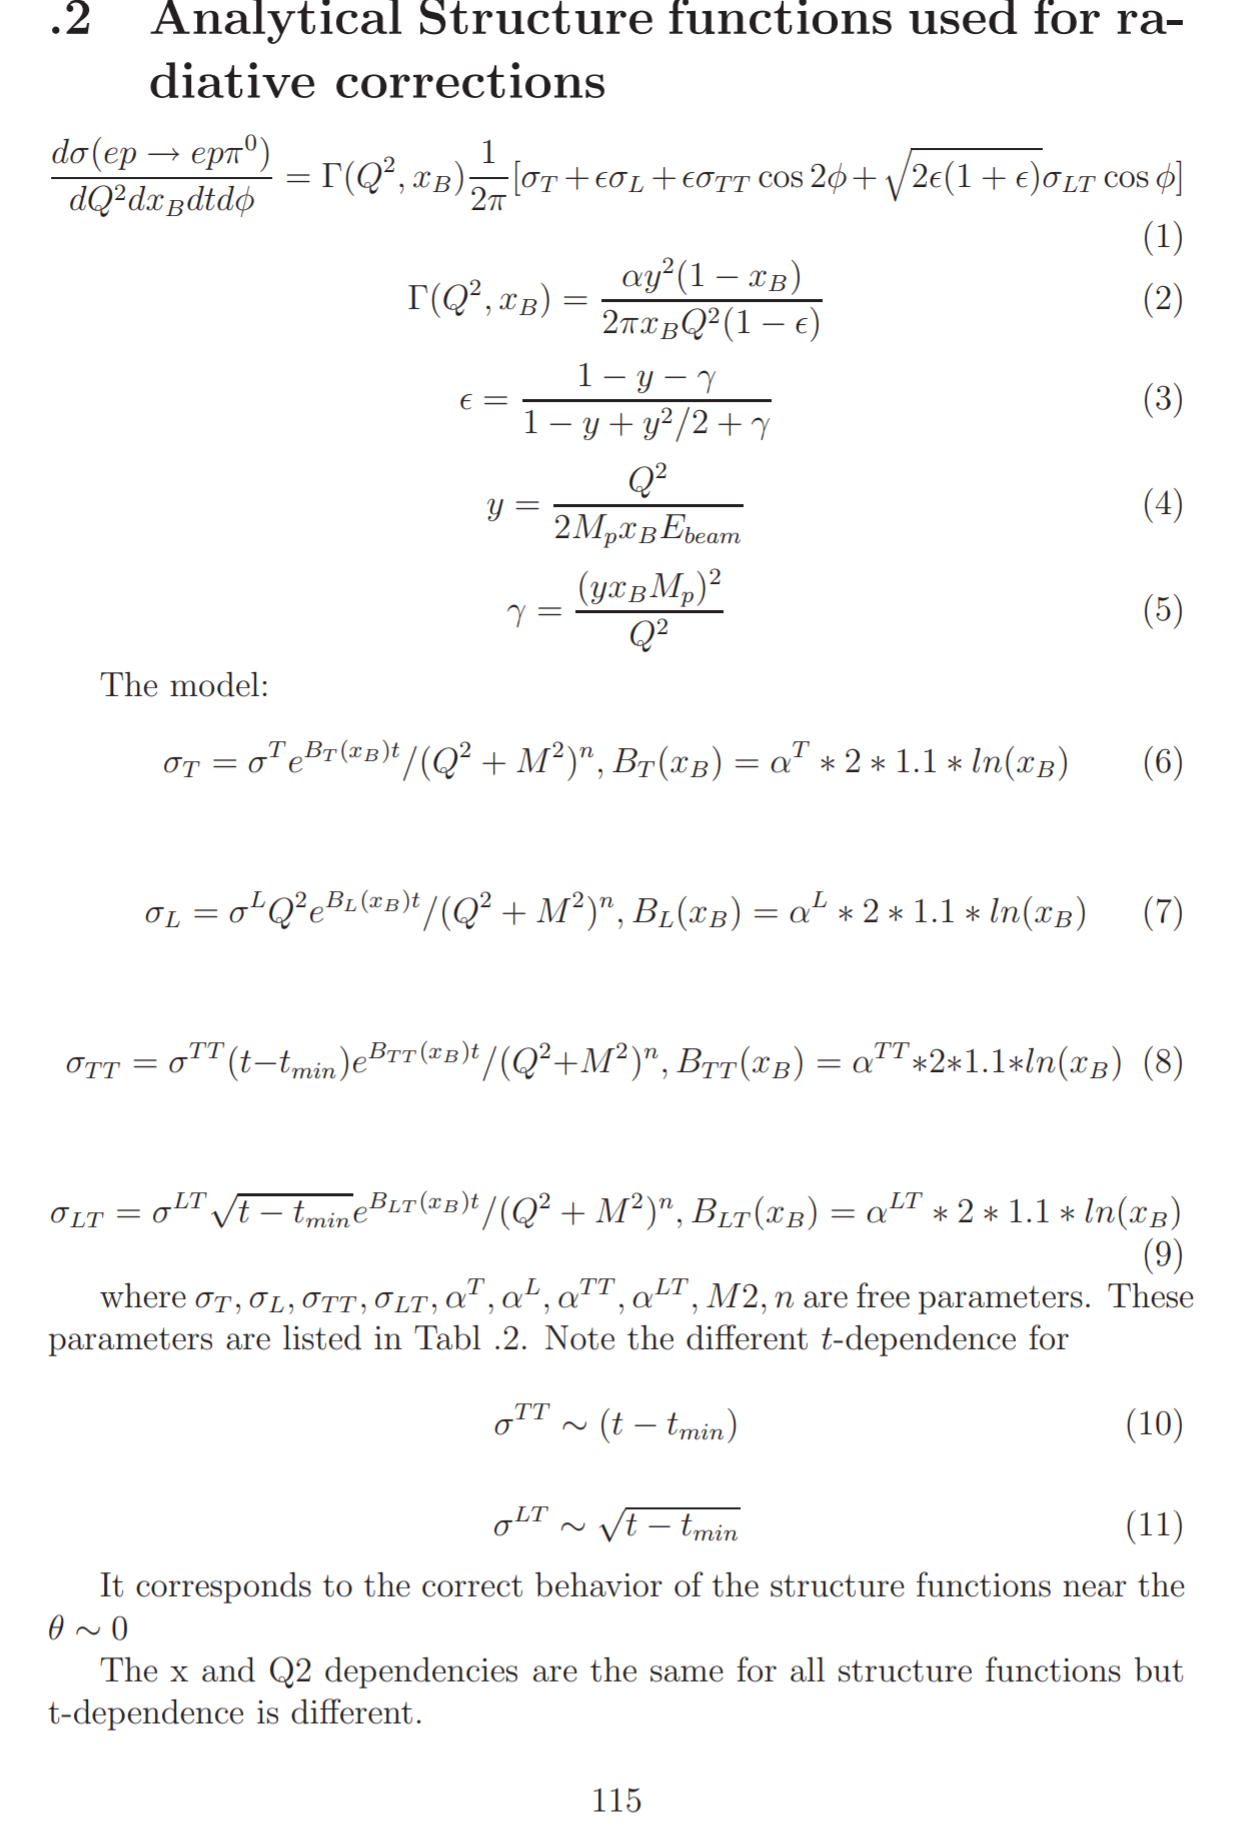
\includegraphics[scale=0.4]{radCorCLAS6.png}
    \caption{Caption}
    \label{fig:my_label}
\end{figure}




\end{document}

\iffalse



Dear All,

I assembled a wikipage to document the minutes of our first and future meetings, this can be found under the "Minutes" tab. Additional tabs are designed to document each member's respective work under the category their work falls under. If I missed a member or if you did not submit your presentation please email me.

https://clasweb.jlab.org/wiki/index.php/DVCS/DVMP_Joint_Analysis_Group#tab=Overview








Dear Andrey,

Could you send us a link to the github for aao_rad and aao_norad with some instructions so that Bobby can follow up for his pi0 analysis?  

Dear Bobby,

aao_rad and aao_norad are event generators for exclusive pi0 and pi+ channels with/without radiative effects.  They are written in Fortran.  The program was initially developed by Volker Burkert long time ago for the resonance region, then has been evolved for many years and recently extended to DIS region even though lots of things need to be done.  Try this to see whether it works.  

Thanks.

Best regards, Kyungseon


Dear Stefan,

Could you upload the program (C++ version, perhaps in Githup with some instructions) that Kemal Tezgin recently wrote in order to calculate the pi0/pi+ channel observables based on the most recent GK model calculations?  Thanks.

Best regards, Kyungseon


Dear Kyungseon,

I have attached the program to calculate the single terms of the pi0 
cross-section based on the GK model.
Its only one file and relatively easy to use. The instructions are in 
the first few rows of the file.
The output can be modified in the main routine at the end of the file.

Best regards,
Stefan --- this file is name Pi_GK_Vegas.cpp


Main ToDo:

Hi Bobby,
Please take a look at README:
https://github.com/drewkenjo/aao_norad
It has instructions how to compile, run and configure the program.
Please don't hesitate to ask questions!
Best,
Andrey.

\fi